\documentclass[11pt]{article}

% HW2_G13_report.tex builds the final report; HW2_G13_report_review.tex defines \anonymous and builds the
% anonymised draft for the LLM TA Judge (review mode, Team ID as the only author).
\ifdefined\anonymous
  \usepackage[review]{acl}
  \renewcommand\outauthor{\begin{tabular}[t]{c}\bfseries Team G13\end{tabular}}
\else
  \usepackage[preprint]{acl}
\fi

\usepackage{times}
\usepackage{latexsym}
\usepackage[T1]{fontenc}
\usepackage[utf8]{inputenc}
\usepackage{microtype}
\usepackage{graphicx}
\usepackage{CJKutf8}
\usepackage{enumitem}
\newcommand{\zh}[1]{\begin{CJK}{UTF8}{bsmi}#1\end{CJK}}
% \member{letter}{name}{student ID}: anonymised as ``Member <letter>'' in the review build.
\newcommand{\member}[3]{\ifdefined\anonymous Member #1\else\zh{#2} (#3)\fi}
\usepackage{booktabs}
\usepackage{amsmath}
\usepackage{amssymb}
\usepackage{tikz}
\usetikzlibrary{positioning,arrows.meta}

\graphicspath{{../figures/}}
% Tighter spacing between floats and text (margins and font size are unchanged).
\setlength{\textfloatsep}{12pt plus 2pt minus 2pt}
\setlength{\dbltextfloatsep}{12pt plus 2pt minus 2pt}
\newcommand{\ours}{LvU}

\title{Money Laundering Is Not an Outlier: Detecting Illicit Bitcoin Transactions Without Illicit Labels}

\author{
  \textbf{Team G13} \\
  \zh{李尚哲} 314580057 \quad \zh{呂丞頤} 314580055 \quad \zh{黃駿甯} 314580075 \quad \zh{吳美真} 414551035 \\
  \zh{孫傅康} 112550176 \quad \zh{傅維雨} 112550149 \quad \zh{張凱華} 315554024 \quad \zh{李玠廷} 315554034 \\
  \url{https://github.com/leeshuncher/DataMiningHW2}
}

\begin{document}
\maketitle

\begin{abstract}
Cryptocurrency exchanges must flag laundering transactions, but confirmed illicit labels are scarce and late, while licit ones are cheap.
On the Elliptic Bitcoin graph (203,769 transactions, 49 time steps) we show that illicit transactions are \emph{not} outliers: only 1.7\% exceed a 3$\sigma$ rule versus 22.3\% of licit ones, so one-class detectors rank them \emph{below} normal (test ROC-AUC 0.17).
We therefore train a positive-unlabeled detector (\ours{}) that separates licit from unlabeled transactions and never sees an illicit label.
On a chronological test split, \ours{} reaches PR-AUC 0.546\,$\pm$\,0.024 (8.4$\times$ prevalence) and 82\% precision in its top 100 alerts, matching a supervised GraphSAGE network and recovering 69\% of supervised XGBoost's PR-AUC.
Ablations show that 1\% illicit contamination of the licit labels destroys this gain, and every method fails after a dark-market shutdown.
\end{abstract}

% ---------------------------------------------------------------------------
\section{Introduction}

\paragraph{Scenario and stakeholders.}
Virtual-asset service providers must screen the transactions they touch for money laundering.
Every alert goes to a compliance analyst, who decides whether to freeze funds and file a suspicious-activity report.
A missed laundering transaction (FN) exposes the provider to regulatory penalties; a false alert (FP) costs analyst time from a fixed review budget.
Licit labels come from the provider's own KYC-verified customers and from counterparties attributed to regulated exchanges; analyst capacity fixes the alert budget per period.

\paragraph{Motivation.}
Supervised detectors work well on Bitcoin data \citep{weber2019aml} but need confirmed illicit labels, which arrive late, whereas \emph{normal} labels are cheap (known exchanges are tagged automatically).
One-class models, which treat anomalies as rare points far from normal data \citep{chandola2009survey}, are the natural label-free choice, yet \citet{lorenz2020label} found that they perform poorly and that illicit instances are not outlying.
We quantify this failure, explain it, and turn the explanation into a detector.

\paragraph{Definition of anomaly.}
Our data belong to the \textbf{Graph} category: the unit of detection is one Bitcoin transaction, a node in a payment graph.
A transaction is anomalous if the Elliptic labels attribute it to an illicit entity (scams, malware, ransomware, Ponzi schemes, terrorist organisations); it is normal if attributed to a licit entity (exchanges, wallet providers, miners).
Example normal sample: tx 378120377 (step 16, licit; \texttt{local\_53}$=0.92$, \texttt{local\_55}$=0.45$, in/out degree 0/2).
Example anomaly: tx 232014511 (step 1, illicit; \texttt{local\_53}$=-0.49$, \texttt{local\_55}$=-0.47$, degree 1/1).

\paragraph{Research question.}
\emph{Can a detector fitted without any illicit label rank illicit Bitcoin transactions above licit ones on future time steps, even though illicit transactions are not outliers?}

\paragraph{Contributions.}
(C1) Illicit transactions are less extreme than licit ones (1.7\% vs.\ 22.3\% beyond 3$\sigma$), which inverts outlier detectors (test ROC-AUC 0.17 for Isolation Forest, 0.33 for 3$\sigma$; \S\ref{sec:eda}, \S\ref{sec:results}).
(C2) A licit-vs-unlabeled (\ours{}) detector reaches test PR-AUC 0.546 and P@100 0.82 without illicit labels: far above label-free baselines, on par with a supervised graph neural network, below supervised trees (\S\ref{sec:results}).
(C3) It is robust to the unlabeled pool size but collapses when 1\% of licit labels are wrong (\S\ref{sec:ablation}).
(C4) 42\% of its misses fall after a dark-market shutdown, a blind spot shared with supervised models (\S\ref{sec:analysis}).

% ---------------------------------------------------------------------------
\section{Related Work}

\paragraph{Data category and literature.}
Our data are in the \textbf{Graph} category (transactions are nodes, payment flows directed edges); its key challenge is multi-hop structure, as laundering routes funds through chains of transactions.
\citet{weber2019aml} released Elliptic and compared supervised models on a 70:30 temporal split (Table~\ref{tab:related}); Random Forest on all features beat graph convolutional networks.
EvolveGCN \citep{pareja2020evolvegcn} models the graph sequence over time (illicit F1 0.720 in \citealp{weber2019aml}) and reports that no model recovers after the dark-market shutdown.
\citet{lorenz2020label} found that seven unsupervised detectors reach illicit F1 of at most 0.19 (LOF), and proposed active learning, which matches a supervised baseline with 5\% of the labels.
Positive-unlabeled (PU) learning trains a classifier from one labeled class plus unlabeled data \citep{elkan2008pu,bekker2020pu}; we do not use Deep SAD \citep{ruff2020deepsad}, which trains on labeled anomalies that a provider without confirmed cases lacks.

\begin{table}[t]
\centering\small
\setlength{\tabcolsep}{2.4pt}
\begin{tabular}{@{}lllll@{}}
\toprule
Work & Data & Paradigm & Method & F1 \\
\midrule
\citet{weber2019aml} & Elliptic & sup. & RF, AF & 0.788 \\
\citet{weber2019aml} & Elliptic & sup. & GCN & 0.628 \\
\citet{weber2019aml} & Elliptic & sup. & EvolveGCN & 0.720 \\
\citet{lorenz2020label} & Elliptic & unsup. & LOF (best) & $\le$0.19 \\
\citet{lorenz2020label} & Elliptic & unsup. & IF & $\le$0.01 \\
\midrule
Ours & Elliptic & PU & \ours{} & 0.398 \\
Ours & Elliptic & sup. & RF, AF & 0.541 \\
\bottomrule
\end{tabular}
\caption{Prior results (illicit-class F1; sup./unsup.\ = (un)supervised). Prior work trains on steps 1--34; we train on 1--29 and tune $\tau$ on 30--34 (ours: mean F1 of Table~\ref{tab:main}), so numbers give context, not a direct comparison.}
\label{tab:related}
\end{table}

\paragraph{Positioning and method selection.}
Tier~1 assumes anomalies are extreme in some feature (3$\sigma$ rule) or nothing at all (random score).
Tier~2 assumes illicit mass is over-represented in unlabeled relative to licit data (our \ours{}); we also report the one-class Isolation Forest \citep{liu2008iforest}, which assumes anomalies are easy to isolate.
Tier~3 uses full supervision: Random Forest \citep{breiman2001rf} as in \citet{weber2019aml}, XGBoost \citep{chen2016xgboost}, and a graph neural network.
Graph context enters in two ways: as one-/two-hop aggregates and degree (A4), and through message passing with GCN \citep{kipf2017gcn} or GraphSAGE \citep{hamilton2017graphsage} layers, used both as a supervised reference (T3c) and as the classifier inside \ours{} (T2$''$).
Unlike prior work, we fit without illicit labels, explain \emph{why} outlier detectors invert, and analyse failures per transaction.

% ---------------------------------------------------------------------------
\section{Task Definition and Data}
\label{sec:data}

\paragraph{Data set.}
We use the Elliptic Data Set \citep{weber2019aml,elliptic2019data} (CC BY-NC-ND 4.0; an unmodified copy is in our repository).
It contains $N=203{,}769$ transactions and 234,355 edges in 49 time steps about two weeks apart; edges never cross time steps.
Each node has $D=166$ anonymised features: the time step, 93 local features (LF; e.g.\ fees, input/output counts and volumes) and 72 aggregates over one-hop neighbours (AF).
From the edge list we add in/out degree and two-hop aggregates (mean of the neighbours' AF).
\S1 defines the unit of detection and gives a normal and an anomalous example.

\paragraph{Labels.}
Ground truth comes from a heuristics-based labelling of the entities behind each transaction \citep{weber2019aml}: 4,545 illicit, 42,019 licit, and 157,205 \emph{unknown}.
Labels may be noisy (heuristic, entity-level attribution); unknown transactions contain both classes and are never evaluated, but \ours{} uses them as unlabeled data.
The paradigm is semi-supervised: licit and unlabeled data for fitting, illicit labels only for validation-based selection.

\begin{table}[t]
\centering\small
\setlength{\tabcolsep}{3pt}
\begin{tabular}{@{}lrrrrrr@{}}
\toprule
Split & Steps & Tx & Licit & Illicit & Unknown & Ill./lab. \\
\midrule
train & 1--29 & 120,804 & 23,510 & 2,871 & 94,423 & 10.9\% \\
val & 30--34 & 15,461 & 2,922 & 591 & 11,948 & 16.8\% \\
test & 35--49 & 67,504 & 15,587 & 1,083 & 50,834 & 6.5\% \\
\midrule
all & 1--49 & 203,769 & 42,019 & 4,545 & 157,205 & 9.8\% \\
\bottomrule
\end{tabular}

\caption{Chronological split shared by all methods.}
\label{tab:data}
\end{table}

\paragraph{Class imbalance.}
Overall, 2.2\% of transactions are illicit; among labeled ones the ratio is 9.8\% vs.\ 90.2\% (1\,:\,9.2), and on the test split 6.5\% (1\,:\,14.4).
A model that predicts ``always licit'' reaches 93.5\% test accuracy with zero recall, so we never report accuracy.
We use threshold-free ranking metrics (PR-AUC) and choose $\tau$ to maximise F1 rather than relying on a 0.5 cut-off.

% ---------------------------------------------------------------------------
\section{Exploratory Feature Analysis}
\label{sec:eda}

All statistics use the training split only (Figure~\ref{fig:eda}).

\begin{figure*}[t]
\centering
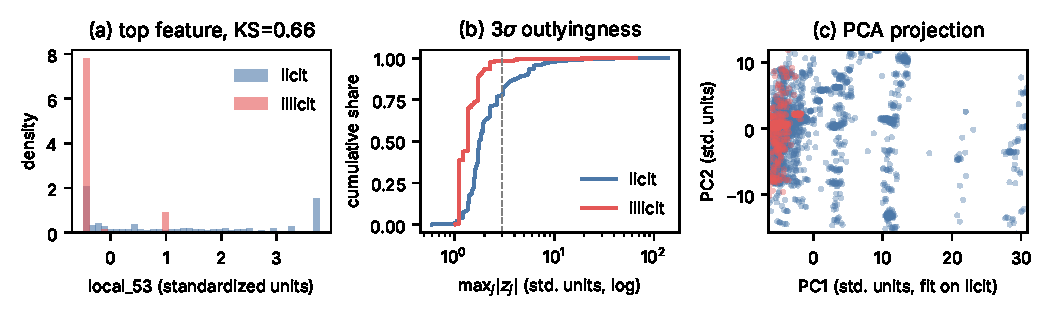
\includegraphics[width=\textwidth]{eda.pdf}
\caption{Training split only. (a) The most separating feature: illicit transactions concentrate on one value. (b) Cumulative share of the largest $|z|$-score (w.r.t.\ licit statistics): illicit transactions are \emph{less} extreme than licit ones; dashed line = 3$\sigma$. (c) PCA fitted on licit data: illicit points form a compact cluster inside the region occupied by licit ones.}
\label{fig:eda}
\end{figure*}

\paragraph{Distribution contrast.}
Figure~\ref{fig:eda}a shows \texttt{local\_53}, the feature with the largest Kolmogorov--Smirnov (KS) distance between classes (0.66, mutual information 0.21 nats).
Most illicit transactions sit on a single value ($-0.49$, shared by 83\% of illicit but 18\% of licit training transactions), whereas licit values spread over the whole range.
Figure~\ref{fig:eda}b is the key observation: only 1.7\% of illicit transactions have any local feature beyond 3$\sigma$ of the licit distribution, against 22.3\% of licit transactions.
In PCA space (Figure~\ref{fig:eda}c), illicit points occupy one compact region; licit points scatter over many clusters.

\paragraph{Separability and redundancy.}
Local features separate the classes better than one-hop aggregates (mean KS 0.38 vs.\ 0.27; 63 vs.\ 30 features with KS $>0.3$; mean MI 0.088 vs.\ 0.060 nats), degree (0.20) and two-hop aggregates (0.18).
89 feature pairs have $|r|>0.95$, and licit behaviour drifts moderately within training (mean KS 0.11, steps 1--14 vs.\ 15--29).
On training edges, 56\% of the labeled neighbours of illicit transactions are illicit (5$\times$ the base rate), but 59\% of all their neighbours are unknown (licit: 46\%).

\paragraph{Hypotheses.}
\textbf{H1}: Outlier-based scores (3$\sigma$, Isolation Forest, Mahalanobis) will rank illicit transactions \emph{below} licit ones.
\textbf{H2}: A model that contrasts licit data with unlabeled data will rank them above, because the compact illicit mode is denser in the unlabeled pool than among labeled licit transactions.
\textbf{H3}: Graph context (aggregates, degree, message passing) will add little, as unknown neighbours dominate.
We test H1--H2 in \S\ref{sec:results}--\ref{sec:ablation} and H3 in \S\ref{sec:ablation}.

% ---------------------------------------------------------------------------
\section{Method}
\label{sec:method}

\begin{figure}[t]
\centering
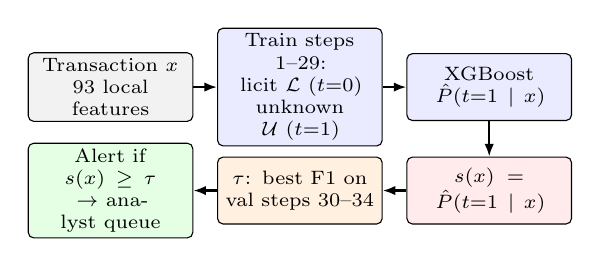
\begin{tikzpicture}[
  box/.style={draw, rounded corners=2pt, align=center, font=\scriptsize, minimum height=0.85cm, inner sep=2pt, text width=1.95cm},
  arr/.style={-{Latex[length=1.6mm]}, thick}]
\node[box, fill=gray!10] (x) {Transaction $x$\\93 local features};
\node[box, fill=blue!8, right=0.3cm of x] (tr) {Train steps 1--29:\\licit $\mathcal{L}$ ($t{=}0$)\\unknown $\mathcal{U}$ ($t{=}1$)};
\node[box, fill=blue!8, right=0.3cm of tr] (m) {XGBoost\\$\hat{P}(t{=}1 \mid x)$};
\node[box, fill=red!8, below=0.45cm of m] (s) {$s(x)=\hat{P}(t{=}1\mid x)$};
\node[box, fill=orange!12, left=0.3cm of s] (tau) {$\tau$: best F1 on\\val steps 30--34};
\node[box, fill=green!10, left=0.3cm of tau] (a) {Alert if $s(x)\ge\tau$\\$\rightarrow$ analyst queue};
\draw[arr] (x) -- (tr);
\draw[arr] (tr) -- (m);
\draw[arr] (m) -- (s);
\draw[arr] (s) -- (tau);
\draw[arr] (tau) -- (a);
\end{tikzpicture}
\caption{\ours{} pipeline. No illicit label is used for fitting; labeled illicit transactions of the validation steps only set $\tau$.}
\label{fig:pipeline}
\end{figure}

\paragraph{Pipeline.}
Figure~\ref{fig:pipeline} shows the Tier~2 pipeline.
The input is the 93 local features of a transaction, used as released (already scaled); the time step is dropped so that the model cannot memorise periods.
We build a training set from the training steps: every labeled licit transaction gets target $t=0$ and every unknown transaction gets $t=1$ (23,510 vs.\ 94,423 rows); illicit training rows are \emph{not} used.
An XGBoost classifier (300 trees, depth 6, learning rate 0.1, row/column subsampling 0.8) learns $\hat{P}(t{=}1\mid x)$.

\paragraph{Anomaly score.}
The score is $s(x)=\hat{P}(t{=}1\mid x)$.
For a well-calibrated classifier, $s$ is monotone in the density ratio $p_{\mathcal{U}}(x)/p_{\mathcal{L}}(x)$.
If the unknown pool is a mixture $p_{\mathcal{U}}=\pi\,p_{\text{ill}}+(1-\pi)\,p_{\text{lic}}$ and labeled licit data follow $p_{\text{lic}}$, the ratio equals $(1-\pi)+\pi\,p_{\text{ill}}(x)/p_{\text{lic}}(x)$ and therefore ranks transactions exactly by how much more likely they are under the illicit than the licit distribution \citep{elkan2008pu}.
Unlike an outlier score, this ranking rewards a dense illicit mode that licit data rarely reach (H2).

\paragraph{Threshold and error costs.}
An FN lets laundered funds pass (regulatory risk); an FP costs analyst time.
With cost ratio $r=c_{\mathrm{FN}}/c_{\mathrm{FP}}$, the cost-optimal $\tau_r$ minimises $r\cdot\mathrm{FN}+\mathrm{FP}$ on the labeled validation transactions (steps 30--34; the test split is never used).
Since $r$ is each provider's choice, all tiers are compared at $\tau_{\mathrm{F1}}$, the validation-F1 maximiser; it behaves like $r\approx1$, so it does \emph{not} encode a costlier FN, and \S\ref{sec:ablation} shows how alerts and recall grow with $r$.

% ---------------------------------------------------------------------------
\section{Experimental Setup}
\label{sec:setup}

\paragraph{Split and leakage prevention.}
All methods share one chronological split by time step (Table~\ref{tab:data}): train 1--29, validation 30--34, test 35--49, i.e.\ 59/10/31\% of steps and 57/8/36\% of labeled transactions.
One-class models fit licit training rows only; \ours{} fits licit and unknown training rows; supervised models fit labeled training rows.
Scalers (3$\sigma$, LOF, $k$NN) are fit on licit training rows; the test set is scored once per seed.

\paragraph{Configurations.}
\ours{}: feature set $\in$\{LF, AF, AF+degree\}, depth $\in\{4,6,8\}$ and trees $\in\{100,300\}$, chosen by validation PR-AUC (LF, 6, 300; 0.901).
Isolation Forest: 200 trees, \texttt{max\_samples} $\in\{256,2048\}$ (2048, LF).
Random Forest as in \citet{weber2019aml} (50 trees, 50 features per split, AF); XGBoost as \ours{}, on AF.
GNNs (PyTorch Geometric, \citealp{fey2019pyg}): two GCN or GraphSAGE layers, full-batch (edges never cross steps), Adam (learning rate 0.01), early stopping on validation PR-AUC (${\le}$1000 epochs, patience 100); validation picked GraphSAGE, width 64 (of 64/128) and AF for both roles.
Grids span common small/medium settings; Tier~3 reuses Weber's RF and \ours{}'s XGBoost settings, so only supervision differs.
Stochastic methods use 5 seeds; deterministic ones (3$\sigma$, Mahalanobis, LOF, $k$NN ratio) report the std of test PR-AUC over 1,000 bootstrap resamples ($\dagger$). Software: Python 3.13, scikit-learn 1.9 \citep{pedregosa2011sklearn}, XGBoost 3.4, PyTorch 2.14; hardware: 4 vCPUs, 16\,GB RAM, no GPU.

\paragraph{Metrics.}
(1) \textbf{PR-AUC} (average precision) is our primary metric: it ignores the large number of easy true negatives and is informative under imbalance \citep{saito2015prc}; its random baseline equals the prevalence.
(2) \textbf{P@100}, the precision of the 100 highest-scored test transactions, models a fixed analyst budget.
(3) \textbf{F1@$\tau$} evaluates the deployed decision.
ROC-AUC is reported to show inversion ($<0.5$).

% ---------------------------------------------------------------------------
\section{Results}
\label{sec:results}

\begin{table*}[t]
\centering\small
\setlength{\tabcolsep}{2.3pt}
\begin{tabular}{@{}llcccccccc@{}}
\toprule
 & & & & & & \multicolumn{2}{c}{PR-AUC by period} & Fit & Score \\
\cmidrule(lr){7-8}
Tier & Method & PR-AUC & ROC-AUC & F1@$\tau$ & P@100 & steps 35--42 & 43--49 & (s) & ($\mu$s/tx) \\
\midrule
T1a & Random score & 0.065$\pm$0.001 & 0.495$\pm$0.006 & 0.122$\pm$0.000 & 0.060$\pm$0.017 & 0.091 & 0.027 & 0.1 & 0.0 \\
T1b & 3$\sigma$ rule (max $|z|$) & 0.053 & 0.326 & 0.010 & 0.040 & 0.075 & 0.028 & 0.1 & 0.2 \\
\midrule
T2$'$ & One-class Isolation Forest & 0.038$\pm$0.000 & 0.170$\pm$0.008 & 0.121$\pm$0.002 & 0.000 & 0.053 & 0.021 & 0.7 & 11.9 \\
T2 & \textbf{LvU classifier (ours)} & 0.546$\pm$0.024 & 0.865$\pm$0.002 & 0.398$\pm$0.011 & 0.822$\pm$0.020 & 0.743 & 0.025 & 4.6 & 1.5 \\
\midrule
T3a & Random Forest (sup.) & 0.767$\pm$0.003 & 0.891$\pm$0.004 & 0.541$\pm$0.138 & \textbf{1.000} & 0.897 & 0.028 & 5.7 & 2.2 \\
T3b & XGBoost (sup.) & \textbf{0.790$\pm$0.001} & \textbf{0.922$\pm$0.002} & \textbf{0.675$\pm$0.056} & \textbf{1.000} & \textbf{0.914} & 0.036 & 2.8 & 1.7 \\
\multicolumn{2}{l}{\emph{prevalence (= random PR-AUC)}} & 0.065 & & & & 0.092 & 0.025 & & \\
\bottomrule
\end{tabular}

\caption{Test results (labeled transactions of steps 35--49), mean\,$\pm$\,std over 5 seeds; $\dagger$: std over 1,000 test bootstrap resamples for the deterministic 3$\sigma$ rule. F1 uses $\tau_{\mathrm{F1}}$ tuned on validation (3$\sigma$ rule: $\tau=3$). Best per column in bold. Period columns split the test set at the dark-market shutdown (step 43).}
\label{tab:main}
\end{table*}

\paragraph{Main comparison.}
Table~\ref{tab:main} supports H1: the 3$\sigma$ rule and the one-class Isolation Forest rank illicit transactions below licit ones (ROC-AUC 0.33 and 0.17) and fall under the random baseline in PR-AUC.
Their val-tuned $\tau$ degenerates to ``alert on everything'' (F1 0.12).
\ours{} supports H2: PR-AUC rises to 0.546\,$\pm$\,0.024 (8.4$\times$ prevalence) and 82\% of its top-100 alerts are illicit.
Bootstrap 95\% CIs of the PR-AUC gap from \ours{}: random [0.45, 0.51], 3$\sigma$ [0.46, 0.53], IF [0.48, 0.54], RF [$-$0.24, $-$0.20], XGBoost [$-$0.27, $-$0.22], GraphSAGE [$-$0.04, 0.03]; paired $t$-tests over seeds agree ($p<10^{-4}$ except GraphSAGE).

\paragraph{Against Tier 3.}
Supervised trees remain clearly better (XGBoost 0.790, RF 0.767), though \ours{} recovers 69\% of XGBoost's PR-AUC without illicit labels.
The gap is not a feature confound: on LF, as \ours{} uses, RF and XGBoost still reach 0.742 and 0.766 (5 seeds, std $\le$0.002).
It loses because it learns ``unlabeled-like'' rather than ``illicit'': licit transactions resembling the unlabeled mass also score high (\S\ref{sec:analysis}).
RF's F1 varies across seeds (0.42--0.80) while its PR-AUC does not: a $\tau$ tuned at 16.8\% validation prevalence transfers poorly to 6.5\% at test.
Trees train in under 6\,s and GNNs in 2--5\,min; all score in 1--12\,$\mu$s per transaction.

\paragraph{Message passing (Graph-specific).}
The supervised GraphSAGE (T3c) reaches PR-AUC 0.552\,$\pm$\,0.035, statistically indistinguishable from label-free \ours{} ($p=0.79$; CI [$-$0.038, 0.027]) and 0.24 below XGBoost, consistent with trees beating GNNs on Elliptic \citep{weber2019aml}.
Inside \ours{}, message passing fails (T2$''$, 0.189): averaging over neighbourhoods dominated by unknown transactions makes most nodes look ``unlabeled'' and erases the licit/unknown contrast (H3).

\subsection{Controlled Ablations}
\label{sec:ablation}

\begin{table}[t]
\centering\small
\setlength{\tabcolsep}{3pt}
\begin{tabular}{@{}lccc@{}}
\toprule
Setting & Test PR-AUC & $\Delta$ & Val \\
\midrule
\multicolumn{4}{@{}l}{\emph{A1: illicit rows hidden in licit side}} \\
\quad 0\% (ours) & 0.546$\pm$0.024 & --- & 0.871 \\
\quad 1\% & 0.142$\pm$0.007 & $-0.404$ & 0.359 \\
\quad 5\% & 0.098$\pm$0.003 & $-0.448$ & 0.247 \\
\quad 10\% & 0.091$\pm$0.004 & $-0.455$ & 0.217 \\
\multicolumn{4}{@{}l}{\emph{A2: fraction of unlabeled pool used}} \\
\quad 5\% & 0.546$\pm$0.018 & $+0.000$ & 0.849 \\
\quad 25\% & 0.520$\pm$0.047 & $-0.026$ & 0.863 \\
\quad 50\% & 0.551$\pm$0.040 & $+0.005$ & 0.833 \\
\quad 100\% (ours) & 0.546$\pm$0.024 & --- & 0.871 \\
\multicolumn{4}{@{}l}{\emph{A3: label-free scoring function}} \\
\quad one-class IF & 0.037$\pm$0.000 & $-0.509$ & 0.108 \\
\quad one-class Mahalanobis & 0.038$\pm$0.001$^\dagger$ & $-0.508$ & 0.097 \\
\quad one-class LOF & 0.190$\pm$0.010$^\dagger$ & $-0.356$ & 0.218 \\
\quad PU $k$NN ratio & 0.194$\pm$0.010$^\dagger$ & $-0.352$ & 0.713 \\
\quad PU classifier (ours) & 0.546$\pm$0.024 & --- & 0.871 \\
\multicolumn{4}{@{}l}{\emph{A4: feature set}} \\
\quad LF, 93 local (ours) & 0.546$\pm$0.024 & --- & 0.871 \\
\quad AF (+72 aggregates) & 0.557$\pm$0.037 & $+0.011$ & 0.768 \\
\quad AF + in/out degree & 0.509$\pm$0.043 & $-0.037$ & 0.756 \\
\quad AF + 2-hop aggregates & 0.536$\pm$0.046 & $-0.010$ & 0.783 \\
\bottomrule
\end{tabular}

\caption{Ablations of \ours{}, one factor at a time: test PR-AUC (5 seeds; $\dagger$ bootstrap std), $\Delta$ vs.\ the full method, and validation PR-AUC (Val, mean).}
\label{tab:ablation}
\end{table}

\begin{table*}[t]
\centering\small
\begin{tabular}{@{}clrrcccl@{}}
\toprule
\# & Type & txId & Step & $s(x)$ & Top-SHAP feature & RF & Likely cause \\
\midrule
1 & FN & 97069571 & 40 & 0.014 & local\_48$=0.09$ & 0.04 & licit-typical profile \\
2 & FN & 73003591 & 42 & 0.970 & local\_53$=-0.49$ & 0.76 & 73/93 features equal \#4 \\
3 & FP & 169360875 & 45 & 1.000 & local\_53$=-0.49$ & 0.03 & licit tx in illicit mode \\
4 & FP & 73160604 & 42 & 0.970 & local\_53$=-0.49$ & 0.41 & 73/93 features equal \#2 \\
\bottomrule
\end{tabular}

\caption{Failure cases of \ours{} (seed 0, $\tau=0.97027$; alert if $s\ge\tau$). RF = supervised Random Forest score (mean of seeds; mean $\tau\approx0.37$). Top SHAP = local feature L$k$ (\texttt{local\_}$k$) with the largest $|$TreeSHAP$|$: value (attribution in log-odds).}
\label{tab:cases}
\end{table*}

Table~\ref{tab:ablation} varies one factor at a time; the configuration was fixed on validation (\S\ref{sec:setup}) before any ablation, and every conclusion also holds on validation (Val).

\paragraph{A1: contamination of the normal labels (AD-specific).}
Replacing just 1\% of the licit training rows with illicit ones (235 rows) cuts PR-AUC from 0.546 to 0.142, far beyond the seed std.
As illicit transactions form one compact mode, a few hundred of them labeled $t=0$ teach the classifier that this mode is ``licit'': \ours{} needs clean licit labels.

\paragraph{A2: size of the unlabeled pool (AD-specific).}
5\% of the unknown pool (4.7k rows) gives the same PR-AUC (0.546); differences stay within one std, so a small unlabeled sample already holds the illicit mode.

\paragraph{A3: scoring function (AD-specific).}
With features and data fixed, outlier scores invert (Isolation Forest 0.037; Mahalanobis with Ledoit--Wolf shrinkage, \citealp{ledoit2004shrinkage}, 0.038), local density scores (LOF, \citealp{breunig2000lof}; a licit/unlabeled $k$NN density ratio) recover some signal (0.19), and the classifier-based density ratio is best (0.546).

\paragraph{A4: graph features (Graph-specific).}
One-hop aggregates ($+$0.011), degree ($-$0.037) and two-hop aggregates ($-$0.010) change test PR-AUC by less than one seed std and lower test F1 (0.30--0.35 vs.\ 0.40), which supports H3; on validation, LF is clearly best (0.871 vs.\ ${\le}$0.783), which is why it was selected.

\paragraph{A5: threshold rule.}
$\tau_{\mathrm{F1}}$ raises 2,459 test alerts (recall 0.65); cost-optimal $\tau_r$ raise 2,333 for $r=1$ (recall 0.64), 3,149 for $r=5$ (0.71), 3,952 for $r=10$ (0.75) and 4,979 for $r=20$ (0.78), all std $\le$0.03.
So $\tau_{\mathrm{F1}}$ acts like $r\approx1$; a provider weighting a miss as ten false alerts should accept 1.6$\times$ more alerts.
The label-free 95th-percentile rule (5,420 alerts, recall 0.80) acts like $r>20$; 30 alerts per step give the best precision, 0.48, at recall 0.20.

% ---------------------------------------------------------------------------
\section{Analysis}
\label{sec:analysis}

\paragraph{Temporal failure.}
We reproduce the observation of \citet{weber2019aml}: after a dark market closes at step 43, every model fails (Table~\ref{tab:main}, period columns).
\ours{}'s F1 drops from 0.50 (steps 35--42) to 0.01 (43--49), and its PR-AUC from 0.743 to 0.025, which equals the prevalence (Table~\ref{tab:main}).
Only 15.6\% of test illicit transactions fall in steps 43--49, but they account for 42\% of the misses of \ours{}.
Of the 398 misses (seed 0, $\tau=0.97027$), 69\% are also missed by supervised RF: the blind spot lies in the data, not in the missing labels.


\paragraph{Failure cases.}
Table~\ref{tab:cases} lists four test errors.
\#1 is a complete inversion ($s-\tau=-0.956$): \texttt{local\_48} (SHAP $-$1.54) and \texttt{local\_53}$=1.81$ ($-$1.53), above 99.6\% of illicit but at the 63rd percentile of licit training transactions, pull its score down; RF misses it too (0.04).
\#2 (FN) and \#4 (FP) fall on either side of $\tau=0.97027$ ($s-\tau=-5.1{\times}10^{-4}$ and $+3.8{\times}10^{-5}$): they share 73 of 93 local features (L2 distance 4.1 vs.\ a median of 10.2 to licit transactions) yet carry opposite labels.
Label noise or entities reusing one wallet software are plausible but unverifiable causes, as Elliptic anonymises entities.
\#3 is a confident FP ($s=0.99995$): a licit transaction on the illicit mode \texttt{local\_53}$=-0.49$ that RF correctly scores 0.03; without illicit labels, \ours{} cannot tell which unlabeled mass is illicit.
\textbf{Shared pattern}: errors stem from overlapping modes and post-shutdown drift, not capacity; the first fix is a few analyst-confirmed labels from the new period (active learning, \citealp{lorenz2020label}).

\paragraph{Interpretability.}
With exact TreeSHAP \citep{lundberg2020treeshap}, globally (mean $|$SHAP$|$ over test illicit transactions), \texttt{local\_53} (0.88 log-odds), \texttt{local\_47} and \texttt{local\_76} (0.56 each) dominate; \texttt{local\_53} is also the top EDA feature, so the model uses the illicit mode of \S\ref{sec:eda}.
For the highest-scored true positive, tx 162428632 ($s=0.99990$, RF 0.94), \texttt{local\_53}$=-0.49$ adds 1.23 log-odds and five other features 0.4--0.9 each.
For an analyst this is a reason to review, not proof.

\paragraph{Practical impact.}
At $\tau_{\mathrm{F1}}$, \ours{} raises 2,459 alerts over 15 steps (${\approx}$164 per two-week step) and catches 65\% (${\approx}$704) of the 1,083 illicit test transactions; 71\% of alerts are false, i.e.\ 2.5 per catch.
With 30 alerts per step (450 in total), \ours{} catches 218 illicit transactions (precision 0.48, 7.4$\times$ random review), supervised RF 239 and XGBoost 245: lacking illicit labels costs ${\approx}$25 catches per 450 reviews, so \ours{} suits cold-start triage.

% ---------------------------------------------------------------------------
\section{Conclusion and Limitations}

\paragraph{Key findings.}
Yes, with qualifications: a detector fitted only on licit and unlabeled transactions ranks illicit Bitcoin transactions far above chance on future steps (PR-AUC 0.546 vs.\ 0.065; P@100 0.82), whereas outlier detectors invert (ROC-AUC 0.17), because illicit transactions form a compact, non-extreme mode.
It matches a supervised GraphSAGE and reaches 69\% of supervised XGBoost's PR-AUC, but it fails after the dark-market shutdown, like every model we tested.

\paragraph{Reflection and future work.}
The decision that mattered most was testing outlyingness in EDA (Figure~\ref{fig:eda}b); starting again, we would do it before implementing any one-class model.
Next steps: (i) query analyst labels for the highest-scoring unlabeled transactions after a drift alarm, to address the post-shutdown misses; (ii) estimate the class prior $\pi$ of the unlabeled pool \citep{bekker2020pu} to calibrate $\tau$ across periods.

\paragraph{Limitations.}
\emph{Data coverage}: one blockchain, 49 two-week steps, heuristic entity-level labels and anonymised features; 77\% of transactions are unlabeled, so scores refer to labeled ones only.
\emph{Assumptions}: \ours{} assumes clean licit labels (A1 shows 1\% noise is fatal) and that the unlabeled pool contains the illicit modes of the future, which fails after the shutdown.
\emph{Graph}: multi-hop structure enters as aggregates and two-layer message passing; deeper or temporal GNNs (e.g.\ EvolveGCN) are untested.
\emph{Generalisation}: the inversion may not hold for genuinely extreme fraud (e.g.\ large one-off thefts).

\paragraph{Deployment considerations.}
\emph{Concept drift}: illicit behaviour changed abruptly at step 43; retrain every few steps and audit a small labeled sample, as scores alone do not reveal a collapse.
\emph{Latency and privacy}: scoring takes ${\approx}1.5\,\mu$s per transaction, far below block times; blockchain data are public, but linking addresses to people falls under data-protection and AML rules.

% ---------------------------------------------------------------------------
\section*{Contributions of Each Member}

{\raggedright\hyphenpenalty=10000
\begin{itemize}[leftmargin=*,itemsep=0pt,parsep=0pt,topsep=2pt]
\item \member{A}{李尚哲}{314580057}: EDA; vetted the topic.
\item \member{B}{呂丞頤}{314580055}: assessed candidate topics.
\item \member{C}{黃駿甯}{314580075}: presentation slides.
\item \member{D}{吳美真}{414551035}: drafted the paper.
\item \member{E}{孫傅康}{112550176}: code, slides, coordination.
\item \member{F}{傅維雨}{112550149}: coordination, review.
\item \member{G}{張凱華}{315554024}: review, topic vetting.
\item \member{H}{李玠廷}{315554034}: obtained the dataset.
\end{itemize}
}

\paragraph{AI usage statement.}
We used Claude Code for code and drafting; the team chose the question and verified every number and citation.

\bibliography{refs}

\end{document}
